\documentclass[twoside,11pt]{article}
\usepackage{jmlr2e}
\editor{}

\usepackage{amsmath}
\usepackage{amssymb}
\usepackage{booktabs}
\usepackage{graphicx}
\usepackage{hyperref}
\usepackage{url}
\usepackage{float}
\usepackage{subcaption}

\hypersetup{colorlinks=true, linkcolor=blue, citecolor=blue, urlcolor=blue}

\graphicspath{{../../plots/rl/}}

\ShortHeadings{Learning to Find Cups}{Schmidt}
\firstpageno{1}

\title{Learning to Find Cups: Reinforcement Learning for a Physical
Ping-Pong Ball Launcher\thanks{Code available at: \url{https://github.com/rschmi3/pong-bot}}}

\author{
  \name Ryan Schmidt \email rschmi3@uwo.ca \\
  \addr Department of Computer Science \\
  Western University
}

\begin{document}

\maketitle

% -----------------------------------------------------------------------------
\begin{abstract}
We present \textbf{Pong-Bot}, a physical reinforcement learning system in which
  a Raspberry Pi-controlled 3-axis CNC-style launcher fires ping-pong balls
  across a table to locate cups placed on a $6\times5$ grid. The robot receives
  only directional feedback (\textit{left}/\textit{right}/
  \textit{short}/\textit{long}/\textit{hit}) and has no camera or distance
  magnitude signal, making this a partially observable sequential decision
  problem with a high physical cost per sample. We propose a recurrent policy
  based on a Gated Recurrent Unit (GRU) trained via behavioural cloning (BC)
  from a simple heuristic baseline, followed by REINFORCE fine-tuning. The GRU
  integrates direction history across shots within an episode, enabling more
  efficient convergence than the stateless heuristic. In live evaluation over
  30 sessions, the deterministic GRU policy achieves 100\% hit rate with a mean
  of 7.7~shots, compared to 9.3~shots for the heuristic (both 100\% hit rate).
  We further extend the framework with an outer GRU layer that provides warm
  start positions for multi-cup sessions, reporting preliminary results from 16
  live three-cup sessions.
\end{abstract}

% -----------------------------------------------------------------------------
\section{Introduction}

Physical robot learning presents a fundamental challenge: environment
interactions are expensive, noisy, and slow. A robot that must fire a
projectile to locate an unknown target exemplifies this challenge. Each trial
requires mechanical actuation, and the feedback signal is coarse. We study a
concrete instantiation of this problem: a 3-axis CNC-style launcher controlled
by a Raspberry Pi must find the location of a cup placed somewhere on a
$6\times5$ grid of positions on a six-foot folding table. The only feedback
available after each shot is a directional hint, \textit{left},
\textit{right}, \textit{short}, \textit{long}, or \textit{hit}, with no
distance magnitude and no camera. The cup position is unknown at session start,
and the objective is to find it in as few shots as possible.

A simple heuristic policy provides an adequate starting point: it applies fixed
directional corrections and achieves 100\% hit rate. However, it cannot adapt
its step sizes based on accumulated shot history, leaving room for a more
efficient learned policy. Training a policy purely from reward signals without
demonstrations would require far more physical robot interactions than are
practical, since each interaction requires mechanical actuation and physical
setup time. A static supervised model also falls short: with no memory of prior
shots it cannot integrate directional evidence across an episode.

Our approach combines three components. First, the heuristic provides 30
reliable demonstrations that solve the cold-start problem at zero training
cost. Second, we train a GRU policy by behavioural cloning (BC) from these
demonstrations; the GRU's recurrent hidden state integrates directional history
across shots within an episode, enabling adaptive behaviour the stateless
heuristic cannot perform. Third, we fine-tune with REINFORCE using collected
GRU episodes, further reducing the number of shots to hit with only a small
amount of additional robot data.

We additionally extend the system with an outer RL layer for multi-cup
sessions. When multiple cups are placed on the table, the outer GRU selects a
starting motor position for the next inner search based on the previous cup's
winning position, providing a warm start in a region of the table not yet
searched.

% -----------------------------------------------------------------------------
\section{Techniques to Tackle the Problem}

\subsection{Related Work}

\paragraph{Sequential search and Bayesian optimisation.}
Bayesian optimisation selects queries to balance exploration and exploitation
over an unknown function; \citet{srinivas2010gaussian} propose GP-UCB, a
principled variant that builds a Gaussian process model of the objective. These
methods require a scalar reward at each query. Our setting provides only a
discrete directional hint per shot, left, right, short, or long, rather than
a scalar value, making standard Bayesian optimisation difficult to apply
directly.

\paragraph{Imitation learning and behavioural cloning.}
BC trains a policy to directly imitate expert demonstrations
\citep{pomerleau1988alvinn}. More sophisticated approaches such as DAgger
\citep{ross2011reduction} address distribution shift by iteratively querying
the expert on states visited by the learner, but require repeated expert access
during training. Since our heuristic demonstrations cover the search space well
and distribution shift is mild, simple BC is sufficient and more practical
given limited robot time.

\paragraph{Recurrent policies for POMDPs.}
In a Partially Observable MDP (POMDP), the agent cannot directly observe the
true environment state and must infer it from a sequence of partial
observations. Our problem is a POMDP: the cup position is never directly
observed, and each shot reveals only a directional hint.
\citet{hausknecht2015deep} demonstrate that replacing a memoryless policy with
an LSTM allows an agent to solve partially observable Atari games by
integrating observation history. \citet{wierstra2010recurrent} show recurrent
policy gradients outperform memoryless policies on POMDPs more generally. We
use a GRU rather than an LSTM because our episodes are short (typically 3-16
shots), and the GRU's simpler single-state architecture trains faster with
fewer parameters while achieving comparable performance on short sequences
\citep{chung2014empirical}.

\paragraph{Policy gradient and REINFORCE.}
REINFORCE \citep{williams1992simple} is a policy gradient algorithm that
updates the policy by reinforcing actions that led to high returns. We apply it
for fine-tuning after BC pre-training, using conservative settings to avoid
overfitting on our small number of collected episodes.

\paragraph{Physical robot RL with limited data.}
PILCO \citep{deisenroth2011pilco} is a model-based RL method that learns a
model of the environment's dynamics to reduce the number of physical
interactions needed. While appealing for physical robots, it requires the
environment to be modelable. In our setting, the mapping from motor position to
directional feedback depends on ballistic physics and mechanical noise, making
it difficult to model reliably. BC from heuristic demonstrations is a more
practical alternative.

\paragraph{Hierarchical RL.}
\citet{kulkarni2016hierarchical} introduce hierarchical deep RL with sub-goal
policies, where a high-level policy sets goals for a low-level policy to
execute. Our outer/inner structure is analogous: the outer GRU provides a warm
start position (high-level) while the inner GRU executes the search from that
position (low-level). Unlike option frameworks, our inner policy is fixed
during outer training, simplifying the learning problem.

% -----------------------------------------------------------------------------
\subsection{Method}

\paragraph{Problem as MDP.}
We formulate cup finding as a sequential decision problem with a fixed maximum
number of steps. The state at step $t$ is an 8-dimensional vector: normalised X
and Y motor positions (each divided by 50{,}000 steps), a 4-dimensional one-hot
direction encoding $[\text{left}, \text{right}, \text{short}, \text{long}]$
(all zeros at episode start before the first shot), a binary flag indicating
whether the current shot scored a hit, and a normalised shot counter. Actions
are continuous delta steps $(\Delta x, \Delta y)$ added to the current motor
position. Episodes terminate on a hit or a configurable maximum shot count.

\paragraph{GRU policy architecture.}
The policy is a single-layer GRU with input dimension 8 (matching the state
vector above), hidden dimension 64, and a linear output head producing
2-dimensional normalised deltas. The hidden state persists across shots within
an episode, allowing the policy to maintain a running belief about the cup's
location. At evaluation time the policy outputs a deterministic action; during
data collection, small Gaussian noise ($\sigma \in \{0.005, 0.01\}$) is added
to the output to encourage exploration. In both cases the output is scaled back
to motor steps before execution.

\paragraph{Behavioural cloning training.}
We collect 30 heuristic sessions (all hits, 2-16 shots each) and train the GRU
to match the heuristic's actions using L1 loss. L1 is preferred over MSE
because early-episode corrections are large, and MSE's quadratic penalty would
push predictions toward a conservative average. Two augmentations improve
generalisation: (1) random horizontal flip ($p{=}0.5$), which mirrors the table
geometry and doubles the effective dataset size; (2) an auxiliary loss that
penalises actions moving in the wrong direction relative to the hint. Training
uses Adam with adaptive learning rate scheduling for approximately 200 epochs.

\paragraph{REINFORCE fine-tuning.}
After BC pre-training, we apply one round of REINFORCE using all collected GRU
sessions as training data. Each shot receives a reward of $+1$ on a hit and
$-0.05$ otherwise; returns are discounted with $\gamma{=}0.95$ and normalised
within each episode. We use 5 epochs at learning rate $10^{-5}$. A second
REINFORCE round consistently degraded performance, a sign of overfitting on the
small number of episodes, so the final pipeline is BC followed by a single
REINFORCE round.

\paragraph{Offline evaluation.}
To validate policies without physical robot access, we implement an offline
simulator that replays known cup positions against a policy. Directional
feedback is computed geometrically by comparing each shot's motor position to
the stored cup position, eliminating mechanical noise. This allows rapid policy
evaluation and hyperparameter selection without robot time.

\paragraph{Outer RL extension.}
For multi-cup sessions, an outer GRU provides a warm start position for each
inner search based on the previous cup's winning motor position. The outer
policy is initialised via BC on 500 synthetic episodes, each consisting of 3
distinct cup positions drawn from the heuristic inner session records, then
fine-tuned on live sessions where both the inner and outer policies are
GRU-based.

\subsection{Heuristic Baseline}

The heuristic policy implements a coarse-to-fine binary-search strategy. For
each direction hint it applies a fixed correction:
$\text{left}{\to}{+}\Delta_x$, $\text{right}{\to}{-}\Delta_x$,
$\text{short}{\to}{+}\Delta_y$, $\text{long}{\to}{-}\Delta_y$, with step sizes
decreasing over the course of the episode. The X and Y axes are corrected
independently. The policy is fully deterministic, requires no training data,
and serves as both the performance baseline and the data source for BC.

% -----------------------------------------------------------------------------
\section{Evaluation}

\subsection{Inner Policy: Live Sessions}

We evaluate three policy configurations on live sessions targeting single cups
drawn from the $6\times5$ grid. Table~\ref{tab:inner} summarises results.

\begin{table}[H]
\centering
\caption{Inner policy live session results.}
\label{tab:inner}
\begin{tabular}{lrrrrrrr}
\toprule
Policy & N & Hit\% & Mean & Med & Std & Min & Max \\
\midrule
Heuristic              & 30 & 100\% & 9.3 & 9.0 & 4.2 & 2 & 16 \\
GRU ($\sigma{>}0$)     & 36 & 83\%  & 10.1& 9.0 & 4.1 & 3 & 19 \\
GRU ($\sigma{=}0$)     & 30 & 100\% & 7.7 & 7.0 & 3.5 & 3 & 16 \\
\bottomrule
\end{tabular}
\end{table}

The GRU policy at $\sigma{=}0$ matches the heuristic's 100\% hit rate while
reducing mean shots from 9.3 to 7.7, a 17\% reduction. The exploratory GRU
($\sigma{>}0$) shows an 83\% hit rate and higher mean shots, consistent with
exploration noise degrading precision on some sessions.

\begin{figure}[H]
  \centering
  \begin{subfigure}[t]{0.48\textwidth}
    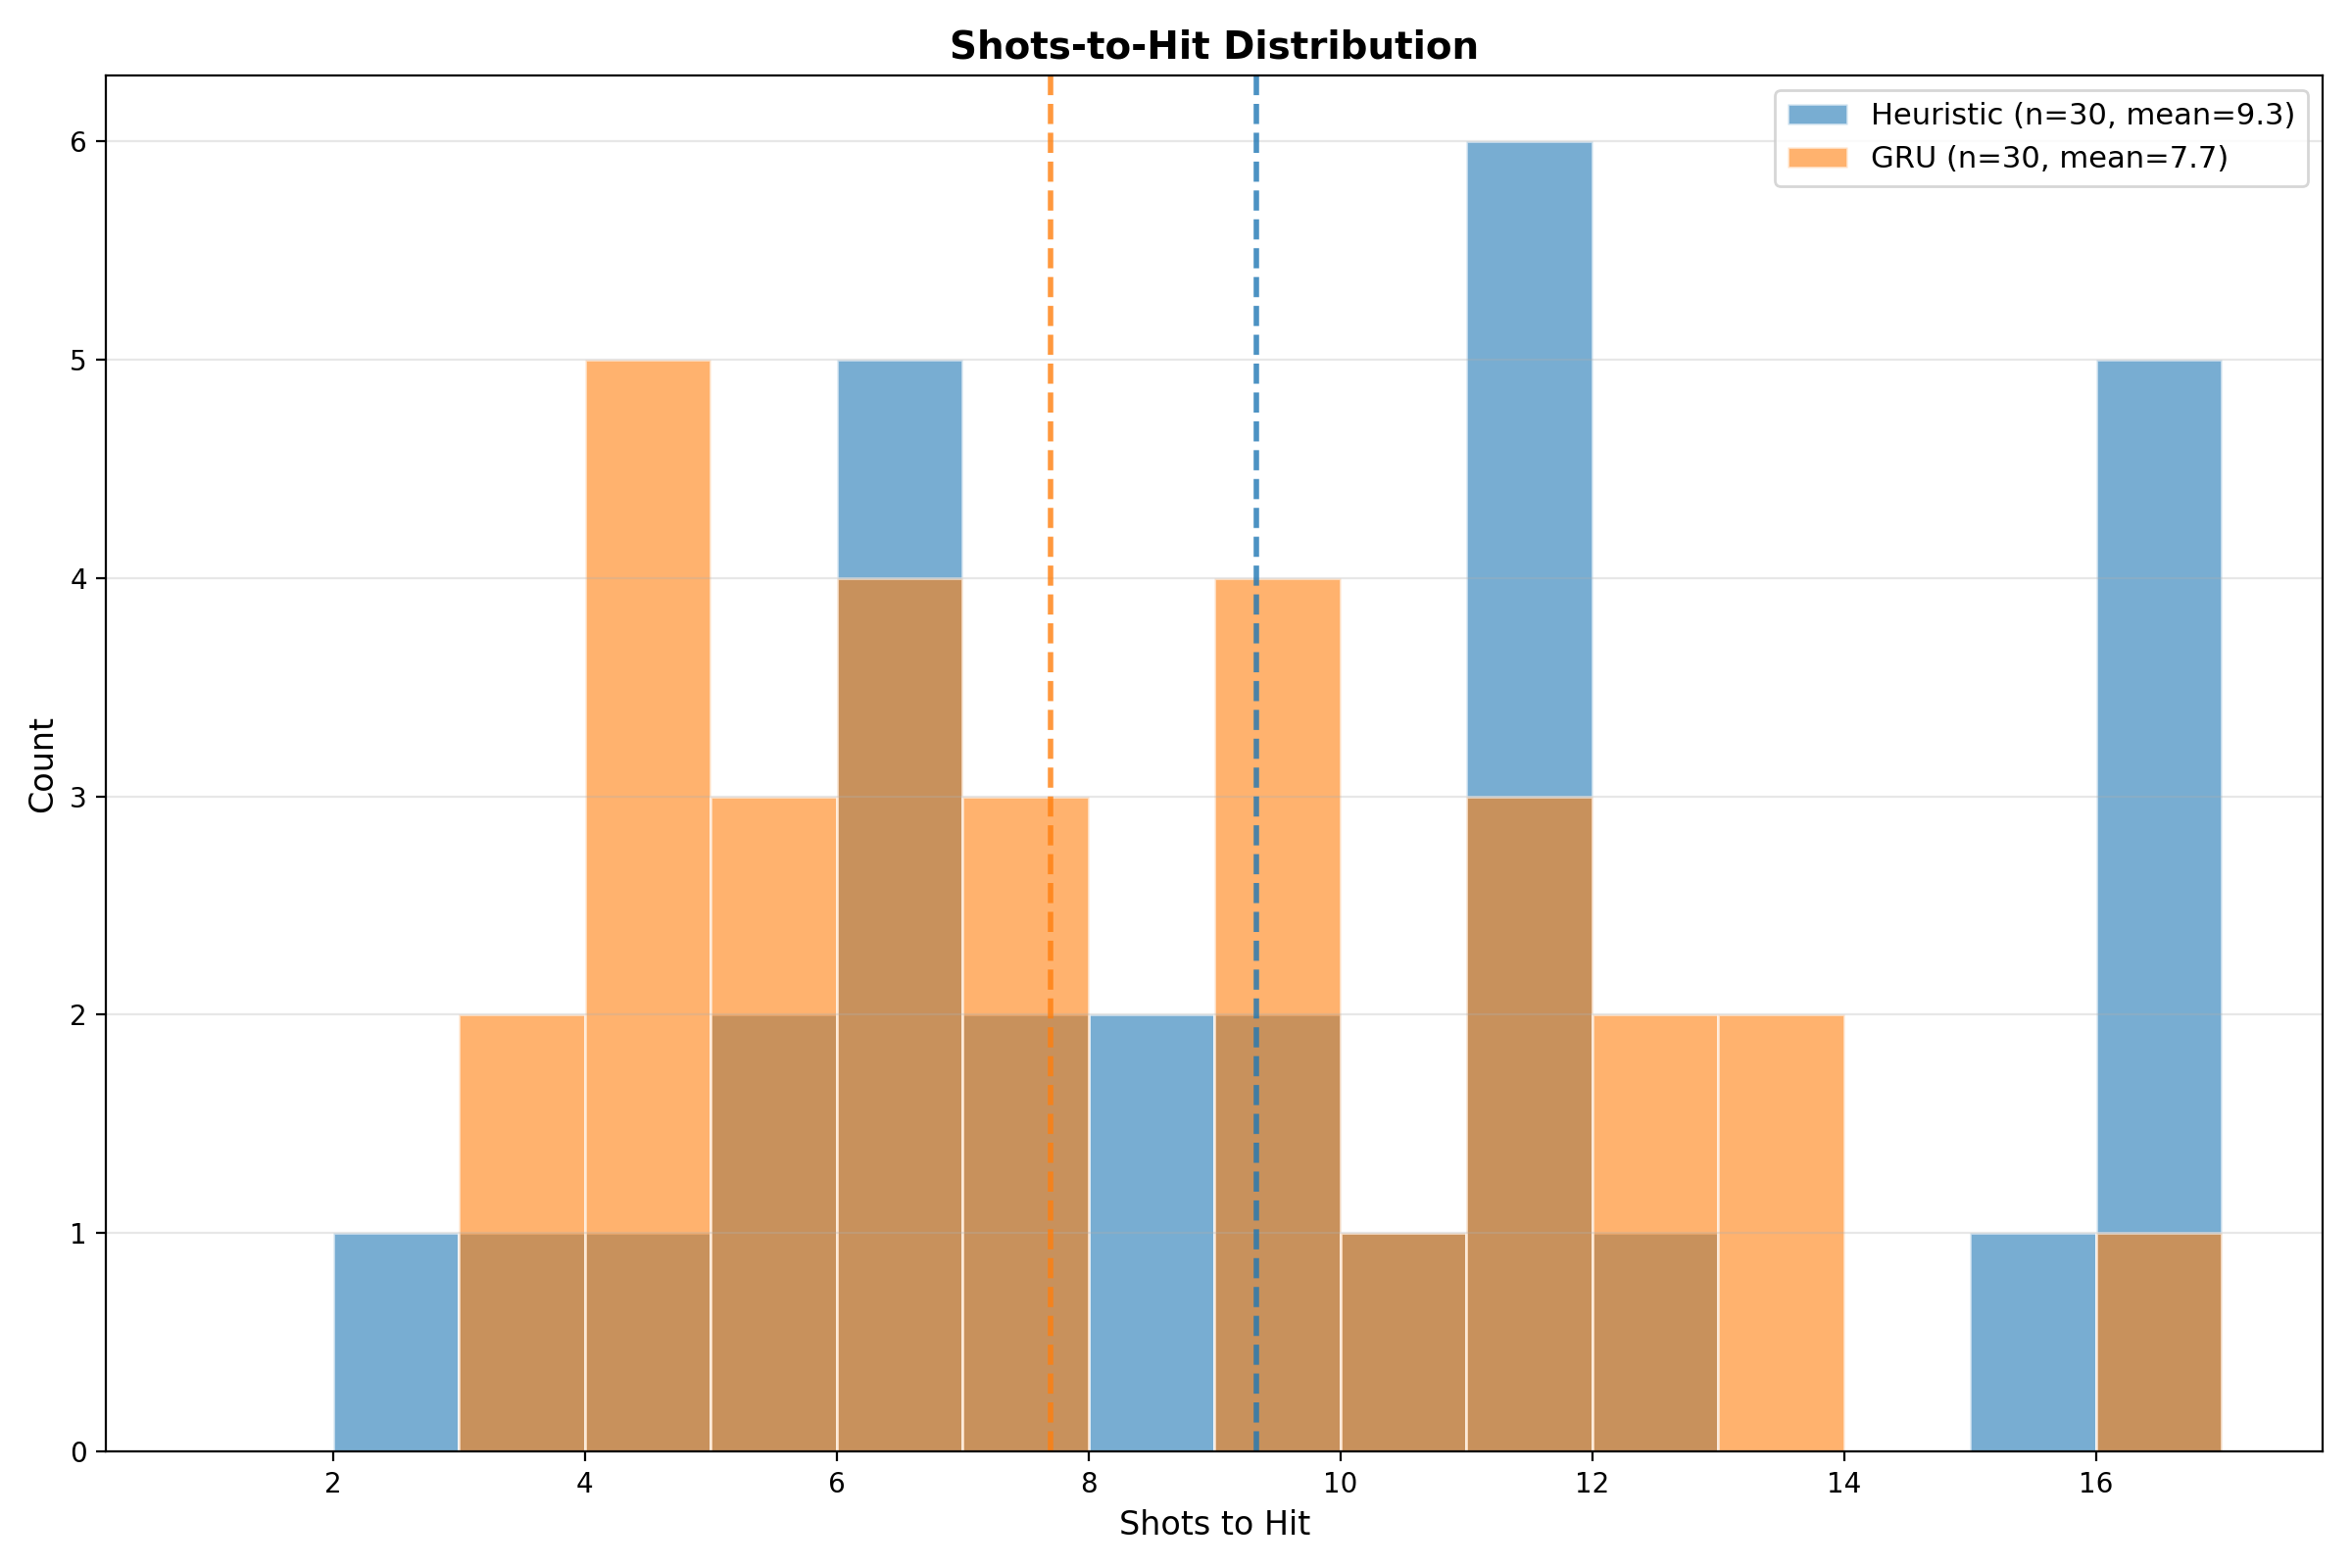
\includegraphics[width=\textwidth]{shots_histogram.png}
    \caption{Shots-to-hit distribution for heuristic (blue) and GRU
      $\sigma{=}0$ (orange). Dashed lines indicate respective means.
      The GRU distribution is shifted left, with more mass at 4--7 shots.}
    \label{fig:hist}
  \end{subfigure}
  \hfill
  \begin{subfigure}[t]{0.48\textwidth}
    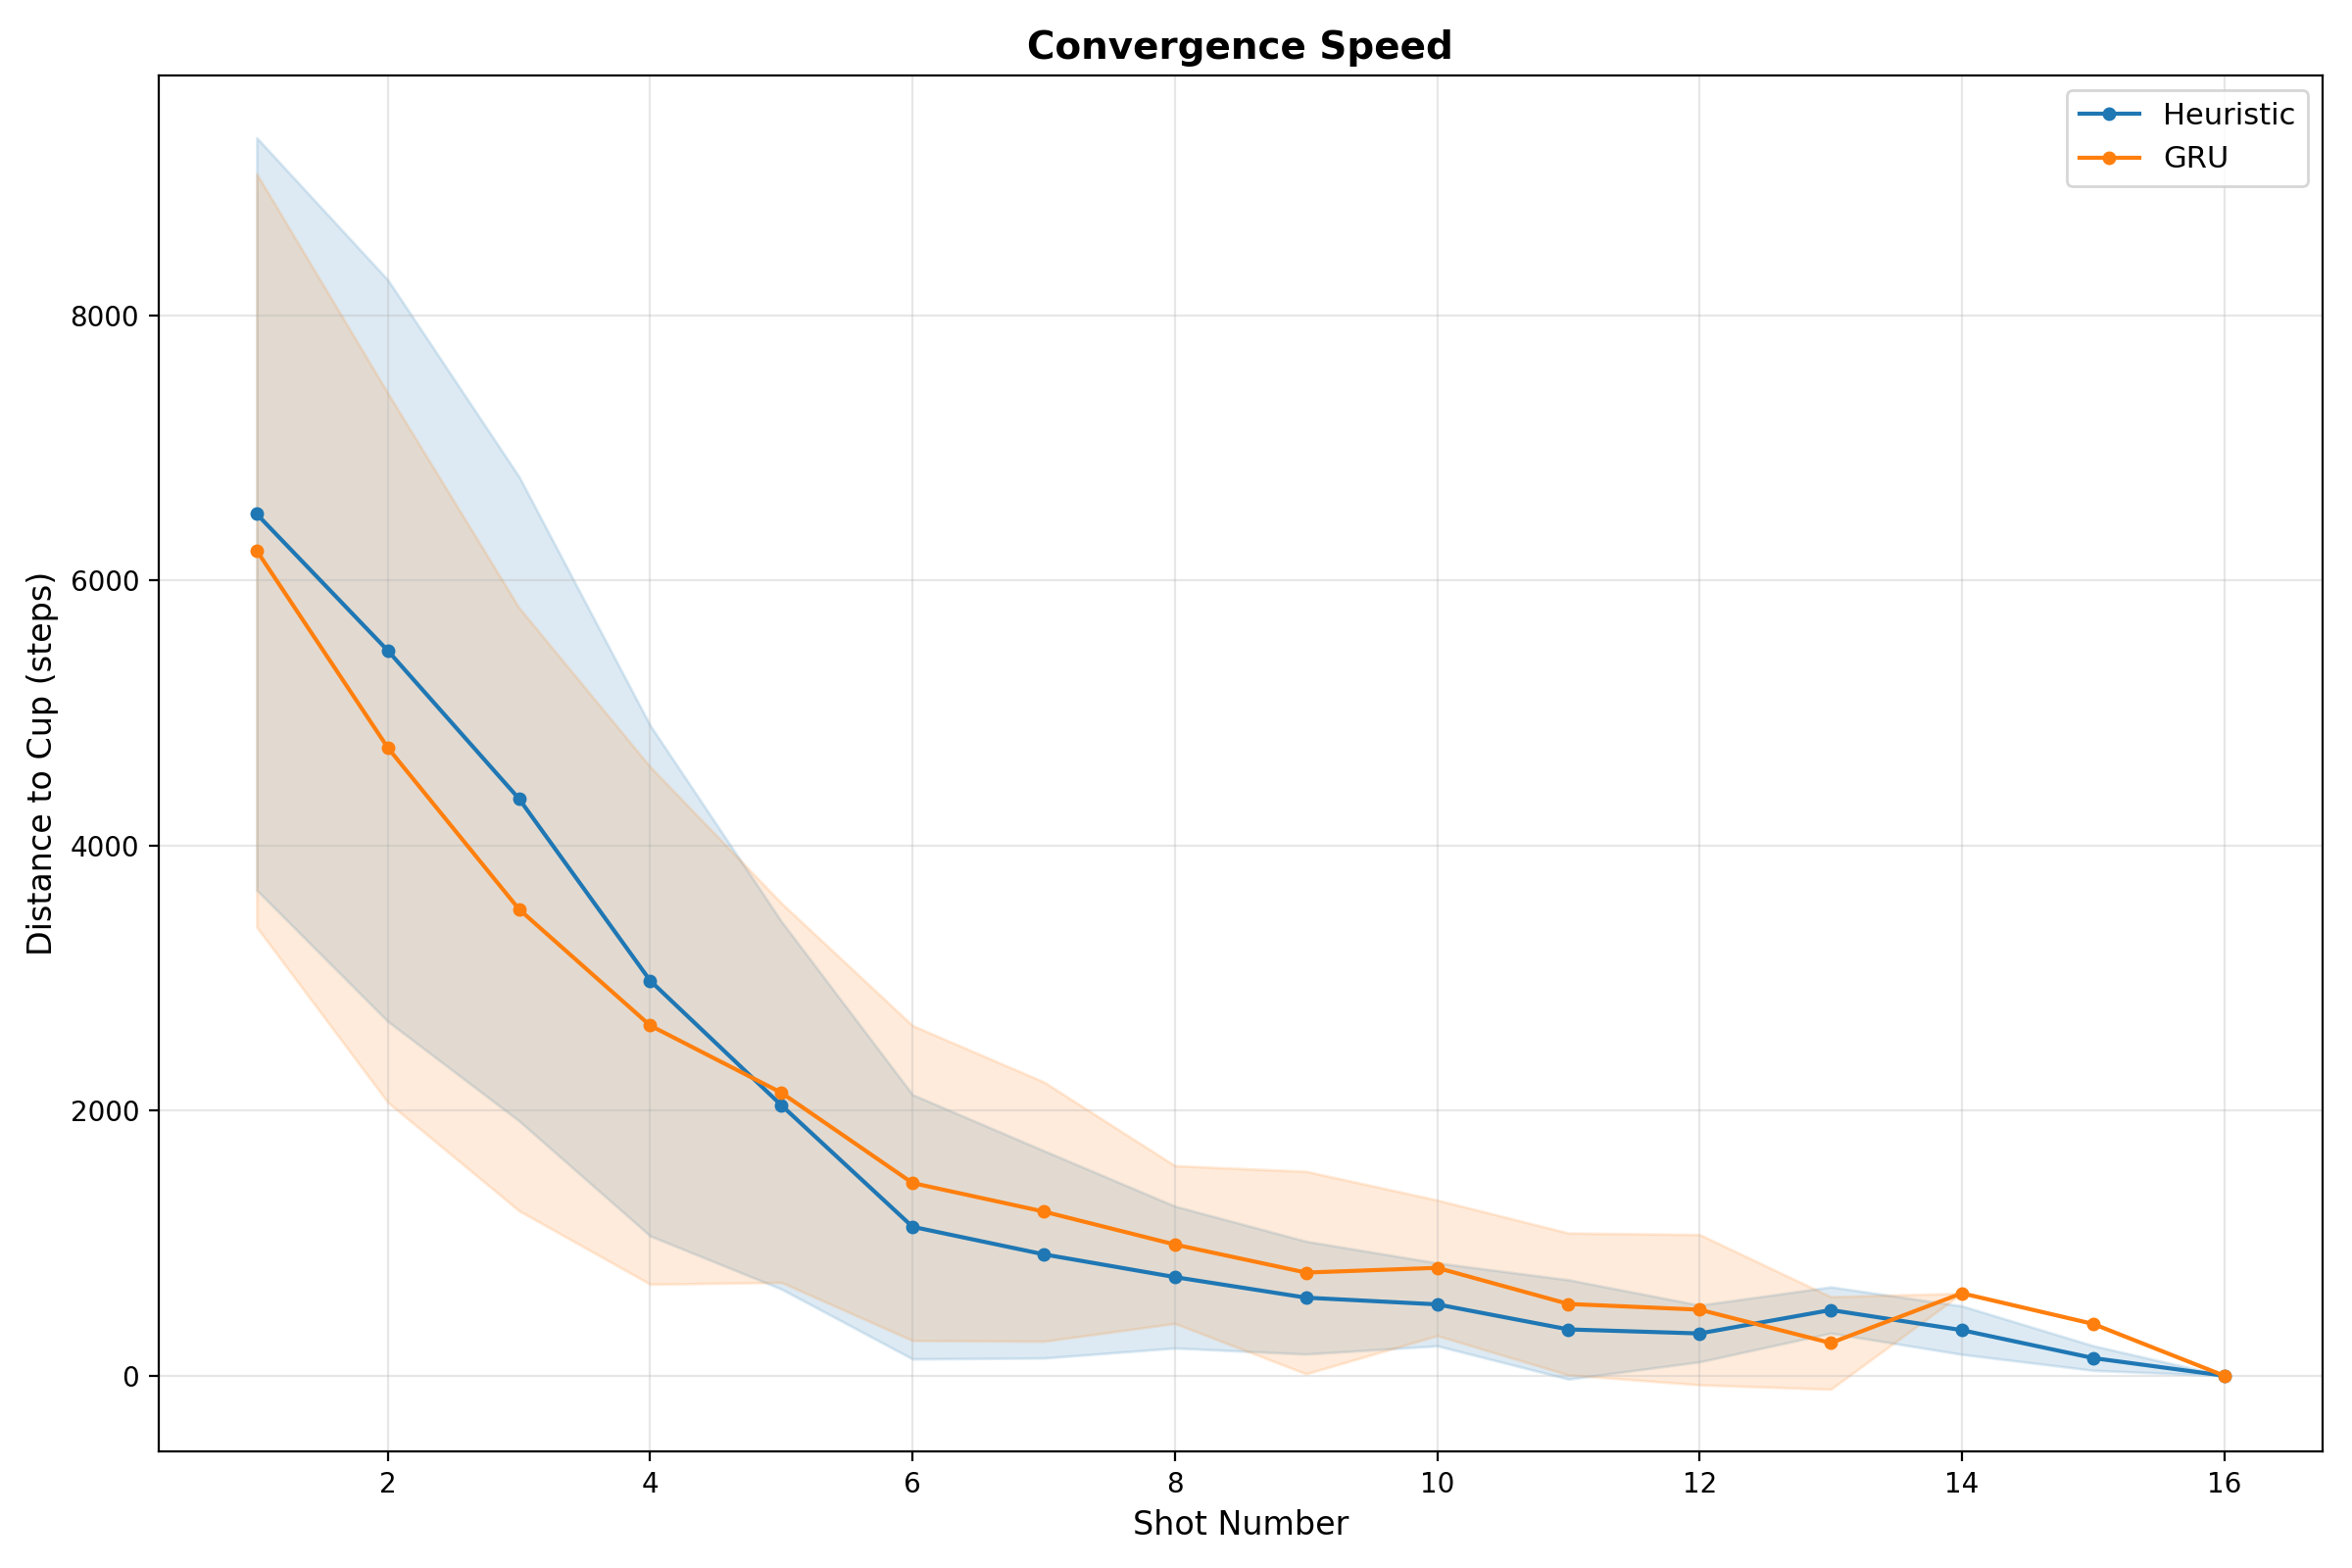
\includegraphics[width=\textwidth]{convergence_speed.png}
    \caption{Mean distance-to-cup (motor steps) vs.\ shot number with
      $\pm1$ std bands. The GRU converges faster in shots 2--5, then
      tracks the heuristic in the fine-convergence phase.}
    \label{fig:conv}
  \end{subfigure}
  \caption{Inner policy performance.}
\end{figure}

\subsection{Offline Simulation}

Table~\ref{tab:sim} reports offline simulation results on the 30 heuristic cup
positions. The simulator computes directional feedback analytically,
eliminating mechanical noise.

\begin{table}[H]
\centering
\caption{Offline simulation results (30 cup positions).}
\label{tab:sim}
\begin{tabular}{lrr}
\toprule
Policy & Hit Rate & Mean Shots \\
\midrule
Heuristic        & 100\% (30/30) & 5.5 \\
GRU $\sigma{=}0$ & 100\% (30/30) & 6.4 \\
\bottomrule
\end{tabular}
\end{table}

In the noiseless simulator the heuristic achieves 5.5 mean shots versus 6.4 for
the GRU. This reversal relative to live sessions suggests that the heuristic's
fixed step-size strategy is well-suited to noiseless conditions, while the
GRU's learned behaviour may provide an advantage on the physical robot where
mechanical variability is present. Directional accuracy in simulation is 100\%
across all four directions (left 14/14, right 56/56, short 7/7, long 85/85).

\subsection{Inner GRU: Trajectory and Coverage}

Figure~\ref{fig:traj} illustrates how the two policies navigate toward a cup
across multiple sessions. The heuristic follows a systematic correction pattern
while the GRU tends to converge more directly, consistent with its lower mean
shots. Both policies achieve 0 timeouts across all 30 sessions, confirming
reliable coverage of the full $6\times5$ grid.

\begin{figure}[H]
  \centering
  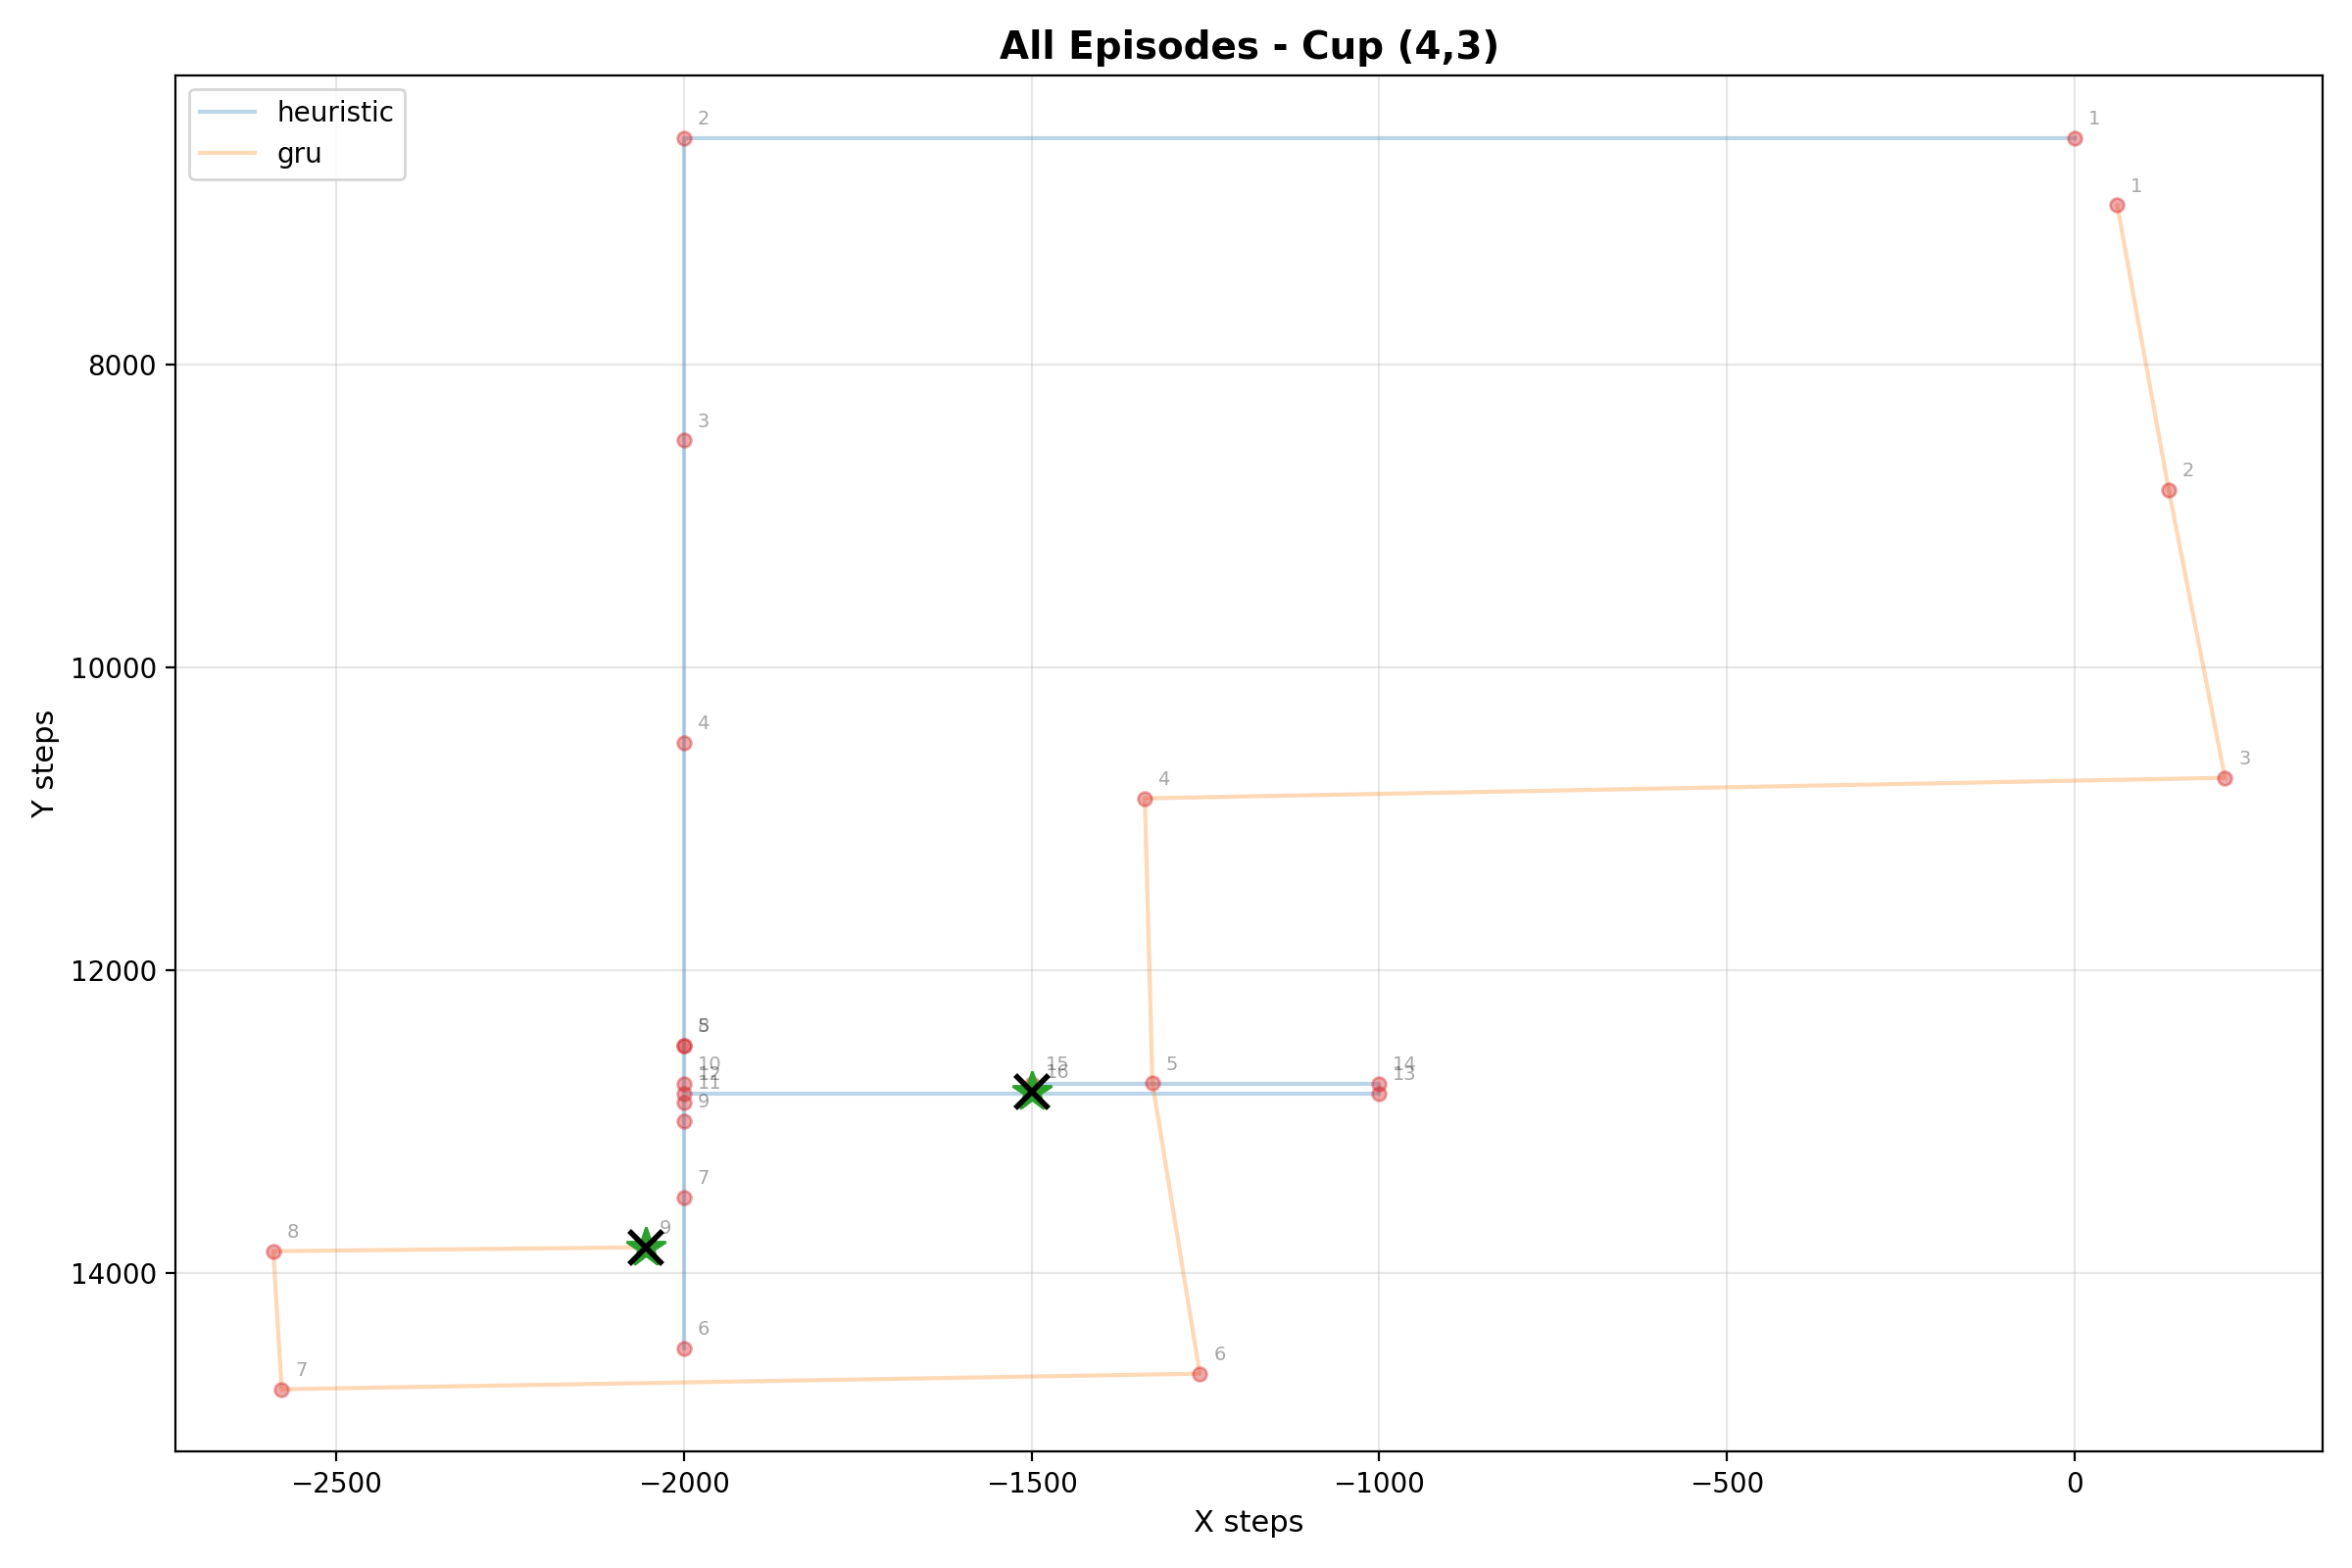
\includegraphics[width=0.7\textwidth]{trajectory_overlay_cup4_3.png}
  \caption{Shot trajectories for all sessions targeting cup (4,3).
    Blue: heuristic; orange: GRU. The GRU takes more direct paths.}
  \label{fig:traj}
\end{figure}

\subsection{Outer RL: Multi-Cup Sequencing}

We evaluate the outer GRU on 3-cup sessions where the inner policy is also
GRU-based, comparing against a simulated heuristic baseline.
Table~\ref{tab:outer} and Figure~\ref{fig:outer} report results. No live
heuristic outer sessions were collected; the baseline is a simulated
distribution of 500 episodes, each consisting of 3 distinct cup positions drawn
from the heuristic inner session records.

\begin{table}[H]
\centering
\caption{Outer RL session results (3-cup sequences).}
\label{tab:outer}
\begin{tabular}{lrrrrr}
\toprule
Configuration & N & Mean & Std & Min & Max \\
\midrule
Heuristic + fixed outer (simulated) & 500 & 28.1 & 6.9 & 10 & 48 \\
GRU + GRU outer (live)              &  16 & 31.2 & 11.2& 12 & 57 \\
\bottomrule
\end{tabular}
\end{table}

\begin{figure}[H]
  \centering
  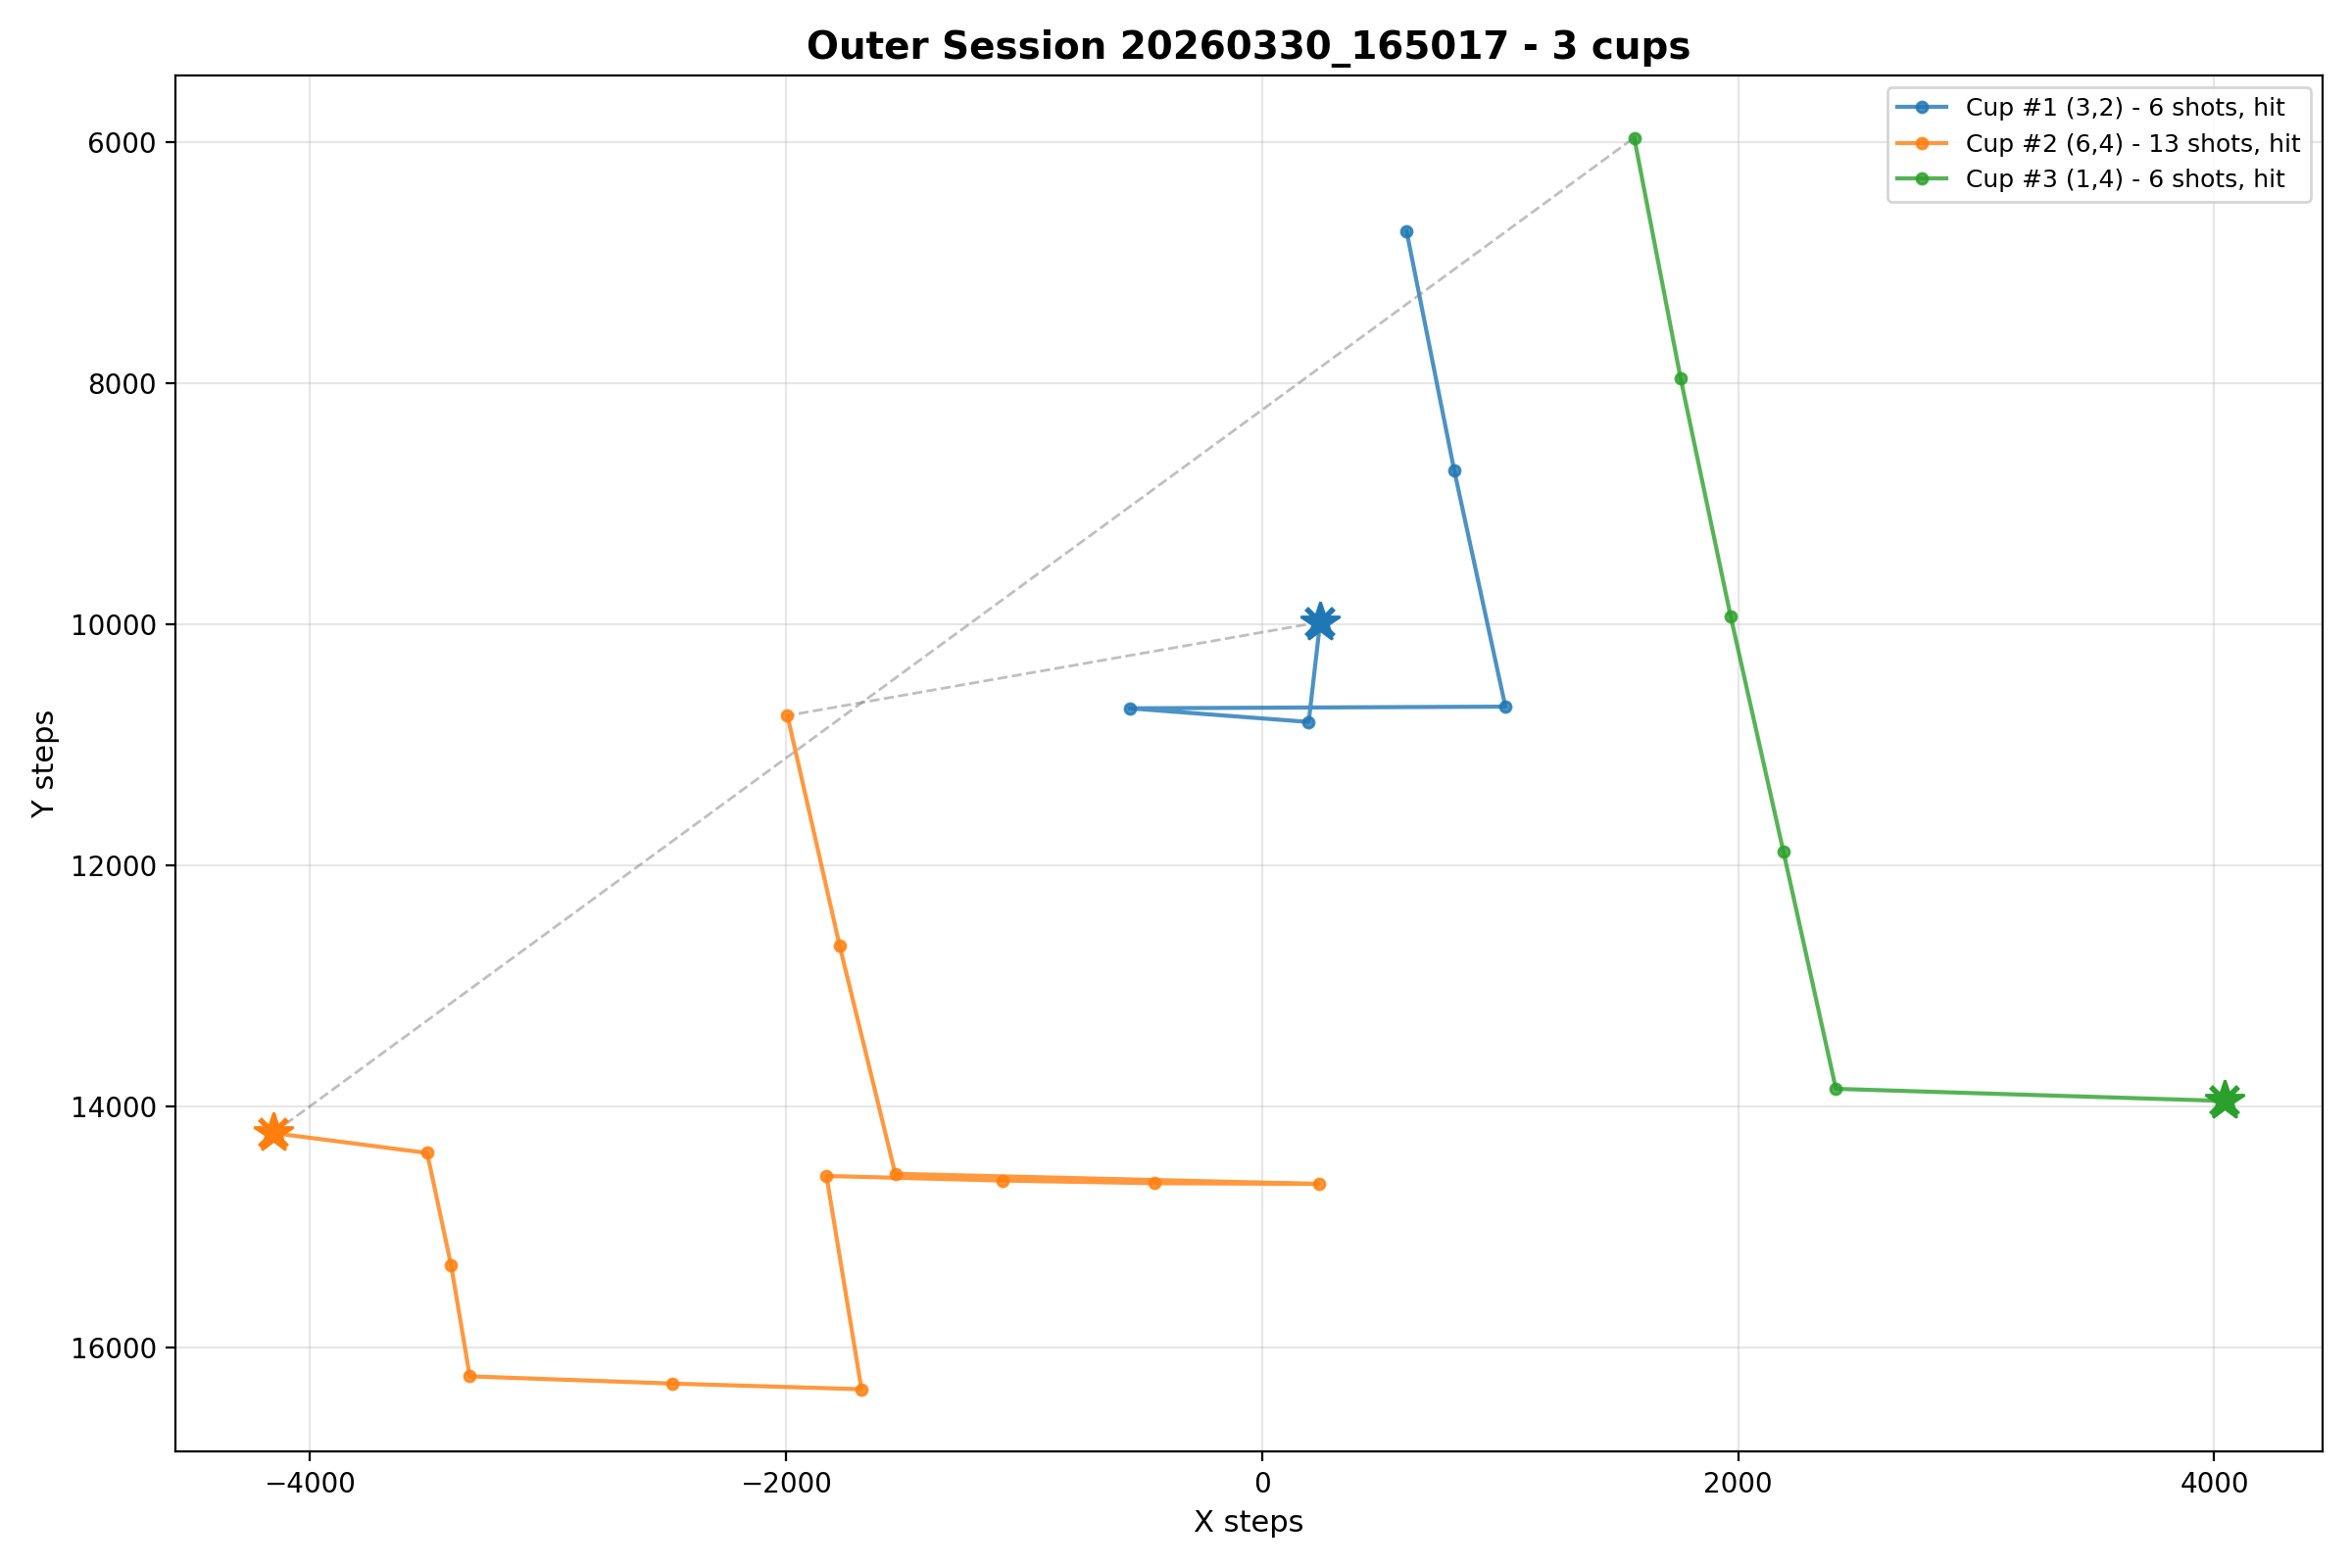
\includegraphics[width=0.8\textwidth]{outer_trajectory_20260330_165017.png}
  \caption{Example 3-cup outer session. Dashed lines show the warm start
    position provided by the outer GRU for each subsequent inner search;
    solid lines show the inner GRU's search trajectory for each cup.}
  \label{fig:outer}
\end{figure}

The live configuration with GRU inner and outer policies (mean 31.2 shots,
$n{=}16$) does not yet beat the simulated heuristic baseline (mean 28.1 shots,
$n{=}500$). This is an early-stage result: the outer GRU has received only 16
live sessions and no REINFORCE fine-tuning. The comparison is further
complicated by different noise profiles, live sessions include mechanical
variability absent from simulation. We expect the gap to close with more data
and REINFORCE fine-tuning.

% -----------------------------------------------------------------------------
\section{Conclusion}

We have presented Pong-Bot, a physical RL system that learns to find cups on a
table by firing ping-pong balls and receiving only directional feedback. The
GRU policy, trained via BC from heuristic demonstrations and fine-tuned with
REINFORCE, achieves 100\% hit rate with 7.7 mean shots on live sessions,
compared to 9.3 mean shots for the heuristic baseline, a 17\% improvement
while maintaining perfect reliability. The BC+REINFORCE pipeline requires only
30 physical robot sessions, showing that a reliable heuristic can substitute
for large amounts of robot time.

The outer GRU extension shows that warm-start sequencing across multiple cups
is feasible. With 16 live sessions, the outer GRU approaches but does not yet
surpass the simulated baseline, indicating the approach is promising but
requires more data.

\paragraph{Limitations.}
The outer RL comparison is limited by different noise profiles between live and
simulated sessions, making direct performance comparison difficult. The inner
policy evaluation relies on 30 sessions, providing limited statistical power
for fine-grained comparisons. Results may not generalise beyond the specific
motor kinematics and table geometry used in this work.

\paragraph{Future work.}
Four directions are most promising. First, collecting more outer GRU live
sessions and applying REINFORCE fine-tuning should close the gap with the
simulated baseline. Second, transformer or other sequence model architectures
could replace the GRU for more expressive history integration. Third, online
adaptation, updating the policy continuously as new sessions are collected,
could reduce the need for periodic offline retraining. Fourth, curriculum
learning, starting with easier central cups and progressively introducing
harder edge positions, may improve both sample efficiency and worst-case
performance.

% -----------------------------------------------------------------------------
\bibliographystyle{plainnat}
\begin{thebibliography}{99}

\bibitem[Chung et al.(2014)]{chung2014empirical}
Chung, J., Gulcehre, C., Cho, K., and Bengio, Y.
\newblock Empirical evaluation of gated recurrent neural networks on sequence
  modeling.
\newblock \emph{arXiv:1412.3555}, 2014.

\bibitem[Deisenroth and Rasmussen(2011)]{deisenroth2011pilco}
Deisenroth, M.~P. and Rasmussen, C.~E.
\newblock {PILCO}: A model-based and data-efficient approach to policy search.
\newblock In \emph{Proc.\ 28th Int.\ Conf.\ Machine Learning (ICML)}, 2011.

\bibitem[Hausknecht and Stone(2015)]{hausknecht2015deep}
Hausknecht, M. and Stone, P.
\newblock Deep recurrent {Q}-learning for partially observable {MDP}s.
\newblock In \emph{AAAI Fall Symp.\ Sequential Decision Making for Intelligent
  Agents}, 2015.

\bibitem[Kulkarni et al.(2016)]{kulkarni2016hierarchical}
Kulkarni, T.~D., Narasimhan, K., Saeedi, A., and Tenenbaum, J.
\newblock Hierarchical deep reinforcement learning: Integrating temporal
  abstraction and intrinsic motivation.
\newblock In \emph{Advances in Neural Information Processing Systems
  (NeurIPS)}, volume~29, 2016.

\bibitem[Pomerleau(1988)]{pomerleau1988alvinn}
Pomerleau, D.~A.
\newblock {ALVINN}: An autonomous land vehicle in a neural network.
\newblock In \emph{Advances in Neural Information Processing Systems
  (NeurIPS)}, volume~1, 1988.

\bibitem[Ross et al.(2011)]{ross2011reduction}
Ross, S., Gordon, G., and Bagnell, D.
\newblock A reduction of imitation learning and structured prediction to
  no-regret online learning.
\newblock In \emph{Proc.\ 14th Int.\ Conf.\ Artificial Intelligence and
  Statistics (AISTATS)}, pp.\ 627--635, 2011.

\bibitem[Srinivas et al.(2010)]{srinivas2010gaussian}
Srinivas, N., Krause, A., Kakade, S., and Seeger, M.
\newblock {Gaussian} process optimization in the bandit setting: No regret and
  experimental design.
\newblock In \emph{Proc.\ 27th Int.\ Conf.\ Machine Learning (ICML)}, 2010.

\bibitem[Wierstra et al.(2010)]{wierstra2010recurrent}
Wierstra, D., Forster, A., Peters, J., and Schmidhuber, J.
\newblock Recurrent policy gradients.
\newblock \emph{Logic Journal of the IGPL}, 18(5):620--634, 2010.

\bibitem[Williams(1992)]{williams1992simple}
Williams, R.~J.
\newblock Simple statistical gradient-following algorithms for connectionist
  reinforcement learning.
\newblock \emph{Machine Learning}, 8(3--4):229--256, 1992.

\end{thebibliography}

\end{document}
